\documentclass[conference]{IEEEtran}
% ========= 日本語対応(LuaLaTeX推奨) =========
\usepackage{luatexja}
\usepackage{luatexja-fontspec}
\setmainjfont{HaranoAjiMincho}
\setsansjfont{HaranoAjiGothic}

% ========= 一般パッケージ =========
\usepackage{amsmath,amssymb}
\usepackage{graphicx}
\usepackage{booktabs}
\usepackage{array}
\usepackage{url}
\usepackage[hidelinks]{hyperref}
\usepackage{cite}

% ========= 図・グラフ =========
\usepackage{tikz}
\usetikzlibrary{arrows.meta,decorations.pathreplacing,calc,patterns}
\usepackage{pgfplots}
\pgfplotsset{compat=1.17}

% ========= タイトル =========
\title{DRAM技術導入とその戦略的位置づけ(1997--2001)\\
\large 酒田FabにおけるDRAM/PSRAMとロジック展開の関連}

\author{%
  \IEEEauthorblockN{三溝 真一 (Shinichi Samizo)}%
  \IEEEauthorblockA{独立系半導体研究者(元セイコーエプソン)\\%
  Independent Semiconductor Researcher (ex-Seiko Epson)\\%
  Email: \href{mailto:shin3t72@gmail.com}{shin3t72@gmail.com}\\%
  GitHub: \url{https://github.com/Samizo-AITL}}%
}

\begin{document}
\maketitle

\begin{abstract}
\textbf{(日本語)}\\
本論文は,1997年から2001年にかけてセイコーエプソン酒田事業所が
三菱電機からの技術移管を通じて \mbox{0.5\,$\mu$m} $\rightarrow$ \mbox{0.35\,$\mu$m} $\rightarrow$ \mbox{0.25\,$\mu$m} の
DRAMプロセスを短期間で習得し,得られた知見を
先端ロジックや高耐圧混載CMOSへ展開して液晶ドライバー製品化に結びつけた
技術的・戦略的過程を,筆者の実体験に基づき整理する。
主要な不良モード(Pause/Disturb Refresh)の物理起源と対策,
量産歩留まりの推移を示し,獲得知見がその後の事業へ
どのように接続されたかを考察する。\\[1ex]

\textbf{(English)}\\
This paper reviews 1997–2001, when Seiko Epson’s Sakata Fab
assimilated DRAM processes (0.5\,$\mu$m → 0.35\,$\mu$m → 0.25\,$\mu$m) transferred from Mitsubishi Electric.
The acquired know-how was extended beyond DRAM to advanced logic
and high-voltage mixed CMOS, leading to LCD driver products.
Key failure modes (Pause/Disturb Refresh), countermeasures, and yield evolution
are summarized based on the author’s on-site experience.
\end{abstract}

\begin{IEEEkeywords}
DRAM, VSRAM/PSRAM, 0.25\,$\mu$m process, retention failure, disturb failure, Sakata Fab, technology transfer, high-voltage mixed CMOS, LCD driver

\hspace{1em}(日本語)DRAM,VSRAM/PSRAM,0.25\,$\mu$mプロセス,リテンション不良,ディスターブ不良,酒田Fab,技術移管,高耐圧混載CMOS,液晶ドライバー
\end{IEEEkeywords}

% ========== 本文開始 ==========
\section{序論}
1997年,当時の半導体産業は \textit{Windows~95} の世界的普及や
Intel Pentium~II の登場を契機として急成長局面にあった。
製造技術面では,8インチウェーハラインと 0.35\,$\mu$m 世代プロセスの
量産化が進展し,DRAM およびロジックLSIの分野で国際競争が激化していた。

セイコーエプソンは山形県酒田市に新たに建設した 8インチFab
(酒田事業所)において,三菱電機からの技術移管を通じ
0.5\,$\mu$m $\rightarrow$ 0.35\,$\mu$m $\rightarrow$ 0.25\,$\mu$m
の三世代DRAMプロセスを短期間で習得した。
その狙いはDRAM事業単独で競争優位を築くことではなく,
DRAMを媒体として最新プロセスを自前化し,
最終的にはロジック/高耐圧混載CMOSや液晶ドライバーに展開する点にあった。

本研究はこの「DRAM導入を目的ではなく手段とする」戦略的枠組みを,
筆者の現場経験に基づき整理する。
特に,立ち上げ初期の不良モード解析(Pause/Disturb Refresh Fail)とその対策,
歩留まり改善,さらに獲得知見がロジック展開に
どう接続されたかを考察する。

\section{第1章:0.5\,\texorpdfstring{$\mu$m}{μm} と 0.35\,\texorpdfstring{$\mu$m}{μm} 世代の立ち上げ}

\subsection{0.5\,$\mu$m 16M DRAM}
酒田Fabにおける最初の量産製品は,0.5\,$\mu$m世代の16M DRAMであった。
熊本Fabで確立されたプロセスを移管したものであり,
設備条件やレシピの親和性が高く,立ち上げは比較的スムーズであった。

\begin{itemize}
  \item 熊本Fab実績の16M DRAMプロセスを忠実に導入
  \item 酒田Fabの8インチ設備との適合性が良好
  \item 初期歩留まりから安定しており,短期間で量産に到達
\end{itemize}

この成功により酒田Fabは「量産可能な生産拠点」であることを社内外に示し,
次世代プロセス挑戦の足場を得た。

\subsection{0.35\,$\mu$m 64M DRAM:洗浄フロー差異と「鏡写し」}
次のステップは0.35\,$\mu$m世代の64M DRAMであった。
筆者が深く関与したのもこのプロジェクトである。

\subsubsection{初期の困難}
1997年秋,試作ロット30ロット以上を投入したが,
いずれもパターン形状が大きく崩れ,SEM測定も困難な状況であった。
熊本Fabでは安定していたプロセスが酒田Fabでは再現できず,
現場は「なぜ動かないのか」という重苦しい空気に包まれた。

\subsubsection{原因究明}
徹底調査の結果,原因はプロセス本質ではなく
\emph{洗浄フローの差異}にあった。
熊本では「硫酸過水→アンモニア過水→塩酸過水」の3段フロー,
酒田では省略して「アンモニア過水→塩酸過水」としていた。
この差異がウェーハ表面状態を変化させ,
後工程のプラズマ処理と干渉して膜厚ばらつきを拡大,
パターン崩れを誘発していた。

\subsubsection{解決と「鏡写し」}
最終的な対応は熊本プロセスの完全な「鏡写し」であった。
すなわちフロー,装置条件,手順を一切省略せず再現。
これにより形状不良は解消し,0.35\,$\mu$m世代の量産化に成功した。

当時のキーワードはまさに「鏡写し」であり,
筆者にとっても30ロット以上の失敗を経て
完全移植で量産を達成した強烈な原体験となった。

\subsection{小括}
\begin{itemize}
  \item 0.5\,$\mu$m世代:熊本実績の忠実移管により安定立ち上げ。
  \item 0.35\,$\mu$m世代:洗浄工程省略が大規模不良の原因。
  \item 「鏡写し」の徹底により歩留まり回復,量産成功。
\end{itemize}

これらの経験は「先端プロセス習得では一切の省略を許さない」という
Fab全体への教訓となり,次世代0.25\,$\mu$mプロセス立ち上げの土台となった.

\section{第2章:0.25\,\texorpdfstring{$\mu$m}{μm} 世代64M DRAMの立ち上げ}

\subsection{SCF方式と初期歩留まり}
1998年,酒田Fabは次世代である0.25\,$\mu$m世代64M DRAMの立ち上げに挑んだ。
ここでも三菱電機が確立していた \emph{Short Cycle Feedback (SCF)} 方式を採用した。
SCFは0.5\,$\mu$m世代から用いられていた,短いサイクルで
評価とフィードバックを繰り返し工程条件を迅速に最適化する手法である。

その結果,本番ロットで約65\%の初期歩留まりを達成できた。
20–30\%から始まるのが一般的な新世代DRAMの初期歩留まりと比べると,
65\%は極めて高い水準であった。

手順は以下であった。
\begin{enumerate}
  \item 移管条件をフロッピーディスク2枚から流動票に展開
  \item 主要工程ごとに形式ロット(約10ロット)を途中止めし形状確認
  \item SEM観察や電気特性評価に基づき条件修正
  \item 本番ロット(3ロット)を全工程通して流し,長期信頼性確認
\end{enumerate}

この方式で短期間に工程条件が整備され,量産に直結した。

\subsection{保持時間モデルと不良モード解析}
初期不良は主として \emph{Pause Refresh Fail} に集中した。
これはリフレッシュを一時停止し,セル保持特性を直接評価する試験である。
試験条件を32\,ms $\rightarrow$ 64\,ms $\rightarrow$ 128\,ms と伸ばすと,
単ビット不良が散発的に増加した。
不良はランダム分布し,ライン欠陥やエッジ集中は見られなかった(Fig.~\ref{fig:failmap})。

保持時間は次式で表される。
\begin{equation}
\tau = \frac{C_{\mathrm{cell}} \cdot V_{\mathrm{cell}}}{I_{\mathrm{leak}}}
\end{equation}
容量 $C_{\mathrm{cell}}$,電圧 $V_{\mathrm{cell}}$ は設計通りであり,
問題はリーク電流 $I_{\mathrm{leak}}$ の増大であった。

解析によりキャパシタ誘電体や構造欠陥は否定され,
主因は \emph{拡散層ジャンクションリーク} と特定された。
フェイルマップでも同一座標で再現性が確認され,
プロセス条件起因の系統的不良であることが明らかになった。
物理的起源を概念的に示したのが Fig.~\ref{fig:dram_cross_section} である。

% --- DRAM断面概念図 ---
\begin{figure}[t]
\centering
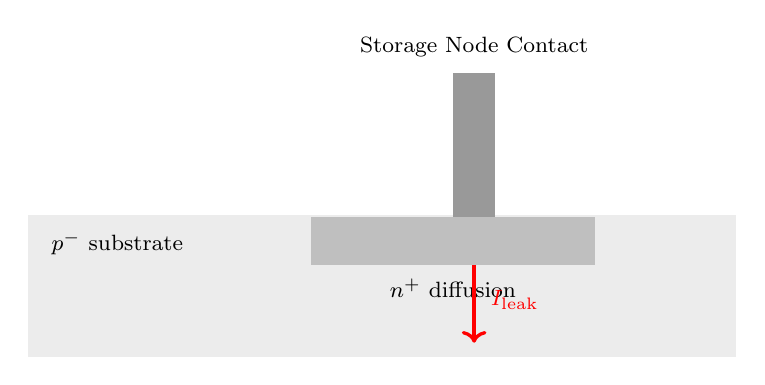
\begin{tikzpicture}[scale=1.8]
\fill[gray!15] (-1,0) rectangle (4,-1.0);
\node[anchor=north west] at (-0.9,-0.05) {\footnotesize $p^-$ substrate};
\fill[gray!50] (1,-0.01) rectangle (3,-0.35);
\node[anchor=north] at (2,-0.38) {\footnotesize $n^+$ diffusion};
\fill[black!40] (2,-0.01) rectangle (2.3,1.0);
\node[anchor=south] at (2.15,1.05) {\footnotesize Storage Node Contact};
\draw[->,very thick,red] (2.15,-0.35) -- (2.15,-0.9);
\node[anchor=west,red] at (2.2,-0.6) {\footnotesize $I_{\mathrm{leak}}$};
\end{tikzpicture}
\caption{DRAM セル断面の概念図(SNコンタクト/$n^+$拡散層/$p^-$基板)。赤矢印は $n^+ \rightarrow p^-$ へのリーク電流 $I_{\mathrm{leak}}$。}
\label{fig:dram_cross_section}
\end{figure}

% --- フェイルマップ ---
\begin{figure}[t]
\centering
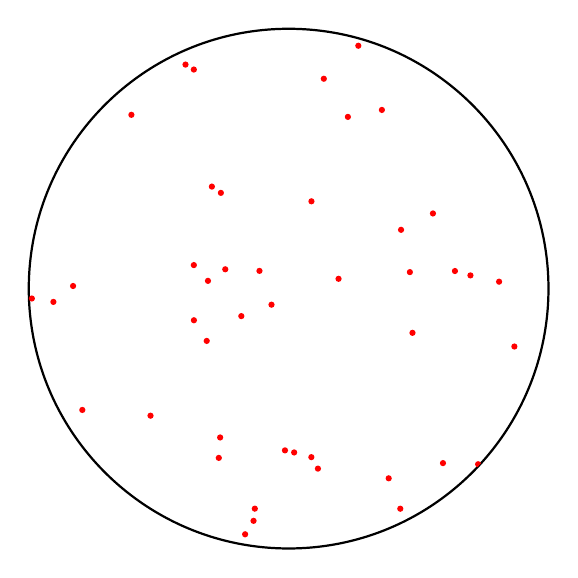
\begin{tikzpicture}[scale=0.22]
  \def\R{15}
  \draw[thick] (0,0) circle (\R);
  \begin{scope}
    \clip (0,0) circle (\R);
    \foreach \i in {1,...,60}{
      \pgfmathsetmacro{\xx}{(rnd*2-1)*\R}
      \pgfmathsetmacro{\yy}{(rnd*2-1)*\R}
      \fill[red] (\xx,\yy) circle (0.18);
    }
  \end{scope}
\end{tikzpicture}
\caption{Pause Refresh Fail のフェイルビットマップ例(ウエハ外周円+ランダム赤点)}
\label{fig:failmap}
\end{figure}

\subsection{プラズマダメージ仮説}
ジャンクションリーク増大の要因として \emph{プラズマダメージ} が浮上した。
特に以下が疑われた。
\begin{itemize}
  \item ゲートエッチ後の酸化膜露出時
  \item LDD工程での繰り返しアッシング
\end{itemize}
酸素プラズマが界面欠陥準位を生成し,熱励起キャリア経路を介して
リーク電流が増加したと推定された。

\subsection{対策と効果}
根本対策は,レジスト剥離を \emph{O$_2$ アッシング} から
\emph{硫酸剥離} に全面切替することであった。
プラズマ曝露を排除し,界面欠陥生成を根本的に防止した。
(低パワー化や再アニールではなく,フローそのものを変更した。)

\begin{table}[t]
  \centering
  \caption{レジスト剥離フローの切替(Before/After)}
  \label{tab:resist_flow}
  \begin{tabular}{p{0.25\linewidth} p{0.65\linewidth}}
    \toprule
    従来(Before) & O$_2$アッシングによるドライ剥離 \\
    対策後(After) & 硫酸剥離によるウエット剥離 \\
    主効果 & プラズマ曝露ゼロ化,界面欠陥・ジャンクションリーク抑制 \\
    歩留まり & 65\% $\rightarrow$ 80\%台後半(Pause改善が支配) \\
    \bottomrule
  \end{tabular}
\end{table}

この切替によりPause Refresh Failは大幅に減少し,
歩留まりは65\%から80\%台後半へ改善した(Fig.~\ref{fig:yield_trend})。

\begin{figure}[t]
\centering
\begin{tikzpicture}
\begin{axis}[
  width=\linewidth, height=6cm,
  ymin=0, ymax=100,
  ylabel={歩留まり(\%)},
  symbolic x coords={0.5\,\mu m,0.35\,\mu m,0.25\,\mu m,VSRAM},
  xtick=data, xticklabel style={align=center},
  xlabel={プロセス世代},
  grid=both,
  legend style={at={(0.5,-0.28)}, anchor=north, draw=none, fill=none,
                /tikz/every odd column/.style={column sep=8pt}, font=\footnotesize},
  legend columns=2, clip=false
]
  \addplot+[semithick,mark=*]
    coordinates {(0.5\,\mu m,95) (0.35\,\mu m,20) (0.25\,\mu m,65) (VSRAM,30)};
  \addlegendentry{初期歩留まり}
  \addplot+[semithick,mark=square*]
    coordinates {(0.5\,\mu m,95) (0.35\,\mu m,86) (0.25\,\mu m,88) (VSRAM,80)};
  \addlegendentry{改善後}
\end{axis}
\end{tikzpicture}
\caption{酒田Fabにおける世代別歩留まり推移}
\label{fig:yield_trend}
\end{figure}

\subsection{小括}
0.25\,$\mu$m世代の立ち上げでは,
SCF方式により迅速な条件整備と65\%という高い初期歩留まりを実現した。
不良の主因はジャンクションリークであり,
プラズマダメージ対策(硫酸剥離への切替)により
80\%台後半へ改善した。
この経験は「表面処理・プラズマ影響を軽視できない」という教訓を残し,
Fabのプロセス自前化に直結した。

\section{第3章:VSRAM(2001年)— Pause/Disturb対策と歩留まり改善}

\subsection{開発背景と初期状況}
2001年,当時の携帯電話市場では「世界初のカメラ付き携帯」の登場が計画されていた。
そのため低消費電力かつ高温動作保証(90\,$^\circ$C)が求められる
新型メモリが必要であった。
酒田Fabでは0.25\,$\mu$m DRAMプロセスを流用し,
内部リフレッシュ制御を追加して \emph{VSRAM(疑似SRAM)} を実現する戦略を採用した。

しかし初期量産歩留まりは約30\%に留まり,
市場投入のタイムリミットを優先して「低歩留まりのまま量産開始」
という厳しい決断が下された。
筆者はこの段階からプロジェクトに参画し,
歩留まり改善を直接担当した。

\subsection{顕在化した不良モード}
VSRAMに特有の不良は以下であった。
\begin{itemize}
  \item \textbf{Pause Refresh Fail}: リフレッシュ停止時に保持時間が不足し,セルデータが失われる。
  \item \textbf{Disturb Refresh Fail}: リフレッシュ動作中のワードライン電圧が隣接セルに影響し,誤反転を引き起こす。
\end{itemize}

Pause Refresh は従来世代でも問題であったが,
Disturb Refresh はモバイル用途での長時間リフレッシュ間隔と
高温保証が重なったことで顕在化した。

\subsection{物理的要因}
Pause Refresh の主因はセルジャンクションリークの増大である。
保持時間モデルに従えば,
\[
\tau = \frac{C_{\mathrm{cell}} \cdot V_{\mathrm{cell}}}{I_{\mathrm{leak}}}
\]
において $I_{\mathrm{leak}}$ が増大すれば $\tau$ は短縮し,
保持不良が顕著になる。
Fig.~\ref{fig:pause_temp_junc} に示すように,
温度上昇とともにジャンクションリーク $I_{\mathrm{junc}}$ は指数的に増加し,
90\,$^\circ$C 条件下で特に顕著であった。
バックバイアスを強化することでリーク増大を抑制できることも確認された。

Disturb Refresh は短チャネル効果(SCE)により
セル間アイソレーションが不十分となり,
ワードライン電圧が隣接セルのしきい値を超えて誤反転を引き起こす現象である。
Fig.~\ref{fig:disturb_temp_sce} に示すように,
チャネル長を短くするとオフリーク $I_{\mathrm{off}}$ が急増し,
温度上昇によりさらに指数的に増大した。
特に90\,$^\circ$C条件下では短チャネルデバイスでの影響が支配的であった。

% --- Pause (温度依存) ---
\begin{figure}[t]
\centering
\begin{tikzpicture}
\begin{axis}[
  width=\linewidth, height=6cm,
  xlabel={温度 [$^\circ$C]}, ylabel={ジャンクションリーク $I_{\mathrm{junc}}$(相対)},
  ymode=log, ymin=1e-2, ymax=1e2,
  xmin=25, xmax=100, xtick={25,40,60,80,90,100},
  grid=both,
  legend style={at={(0.5,-0.22)},anchor=north,draw=none,fill=none},
  clip=false
]
  \addplot+[semithick,mark=*] coordinates {
    (25,0.02) (40,0.06) (60,0.3) (80,1.6) (90,3.2) (100,6.0)
  };
  \addlegendentry{V\_bs=-1\,V}
  \addplot+[semithick,mark=square*] coordinates {
    (25,0.01) (40,0.03) (60,0.12) (80,0.45) (90,0.9) (100,1.8)
  };
  \addlegendentry{V\_bs=-3\,V}
\end{axis}
\end{tikzpicture}
\caption{Pause Refresh:温度上昇で $I_{\mathrm{junc}}$ は指数的に増大。バックバイアス強化で抑制。}
\label{fig:pause_temp_junc}
\end{figure}

% --- Disturb (短チャネル効果) ---
\begin{figure}[t]
\centering
\begin{tikzpicture}
\begin{axis}[
  width=\linewidth, height=6cm,
  xlabel={温度 [$^\circ$C]}, ylabel={トランジスタリーク $I_{\mathrm{off}}$(相対)},
  ymode=log, ymin=1e-3, ymax=1e1,
  xmin=25, xmax=100, xtick={25,40,60,80,90,100},
  grid=both,
  legend style={at={(0.5,-0.22)},anchor=north,draw=none,fill=none},
  clip=false
]
  \addplot+[semithick,mark=triangle*] coordinates {
    (25,0.004) (40,0.01) (60,0.05) (80,0.22) (90,0.45) (100,0.9)
  };
  \addlegendentry{CD=0.25\,\,$\mu$m}
  \addplot+[semithick,mark=*] coordinates {
    (25,0.01) (40,0.03) (60,0.15) (80,0.7) (90,1.4) (100,2.8)
  };
  \addlegendentry{CD=0.20\,\,$\mu$m}
\end{axis}
\end{tikzpicture}
\caption{Disturb Refresh:短チャネル効果で $I_{\mathrm{off}}$ が増大。温度上昇でも指数的に増加。}
\label{fig:disturb_temp_sce}
\end{figure}

\subsection{対策と実装}
不良低減のため,以下の対策を実施した。
\begin{itemize}
  \item \textbf{Pause対策}:
    \begin{itemize}
      \item HF洗浄回数を最小化し,SNコンタクト近傍リークを低減。
      \item バックバイアスを $V_{bs}=-1$\,V $\rightarrow$ $-3$\,Vに強化し,ジャンクションリークを抑制。
    \end{itemize}
  \item \textbf{Disturb対策}:
    \begin{itemize}
      \item ゲートCDを厳密管理し,短チャネルばらつきを抑制。
      \item バックバイアス強化によりしきい値電圧を上昇させ,誤反転を防止。
      \item チャネルドーピング量を増加させ,セル反転耐性を向上。
    \end{itemize}
\end{itemize}

\begin{table}[t]
\centering
\caption{Pause / Disturb 不良に対する主な対策}
\label{tab:pause_disturb}
\begin{tabular}{p{0.18\linewidth} p{0.28\linewidth} p{0.46\linewidth}}
\toprule
不良モード & 主因 & 主な対策 \\
\midrule
Pause   & ジャンクションリーク 
        & HF洗浄制御,バックバイアス強化 \\
Disturb & 短チャネル効果 
        & CD管理,チャネルドーピング,バックバイアス強化 \\
\bottomrule
\end{tabular}
\end{table}

\subsection{効果と歩留まり推移}
対策の結果,
\begin{itemize}
  \item Pause Refresh Fail の発生率が大幅に低下し,内部リフレッシュ間隔延長時でも安定保持可能となった。
  \item Disturb Refresh Fail も90\,$^\circ$C条件下で誤反転が顕著に減少した。
  \item 歩留まりは初期30\%から80\%台へ改善し,量産に耐える水準へ到達した。
\end{itemize}

\subsection{小括}
VSRAM立ち上げでは,モバイル仕様の低消費・高温要求がPause/Disturb不良を顕在化させた。
しかしHF洗浄制御,バックバイアス強化,ゲート寸法管理などにより,
歩留まりは30\%から80\%台へ改善できた。
この成功は酒田FabにおけるDRAM派生製品の集大成であったが,
技術展開はむしろロジック/高耐圧混載CMOSへシフトしていく布石となった。

\section{第4章:0.18\,\texorpdfstring{$\mu$m}{μm} トレンチ系の評価と断念}

\subsection{評価対象と背景}
VSRAM立ち上げ後,次世代候補として
台湾NANYA社の0.18\,$\mu$m DRAMプロセスを利用したVSRAM試作評価が検討された。
NANYAは当時,東芝と技術提携を行っており,
\emph{トレンチキャパシタ方式}をベースとしたプロセスを提供していた。

この評価の目的は,0.25\,$\mu$m DRAM流用VSRAMの後継として,
モバイル用途でさらに高密度・低消費を実現することにあった。

\subsection{技術的特徴}
\begin{itemize}
  \item \textbf{キャパシタ構造}:セルキャパシタはトレンチ型を採用。
        スタック型に比べ面積効率が高い一方,
        ジャンクション面積が大きくリークが増大しやすい。
  \item \textbf{動作仕様}:DRAM標準の80\,$^\circ$C動作保証は満たすが,
        モバイル用途の90\,$^\circ$C保証には設計余裕が少なかった。
\end{itemize}

\subsection{課題の顕在化}
評価の結果,90\,$^\circ$C条件下では以下の問題が顕著に現れた。
\begin{itemize}
  \item \textbf{Pause Refresh Fail}:保持時間不足が多数発生。
  \item \textbf{Disturb Refresh Fail}:高温時に誤反転が増加。
  \item \textbf{高温リーク}:ジャンクション面積拡大に伴いリーク電流が顕著に増加。
\end{itemize}

これらの不良はセル構造に起因し,単純な工程条件調整では改善が困難であった。
特に Fig.~\ref{fig:trench_area_leak} に示すように,
トレンチキャパシタではジャンクション面積の拡大に比例して
ジャンクションリーク $I_{\mathrm{junc}}$ が増加し,
90\,$^\circ$C 条件下では増加率がさらに大きくなることが確認された。

% --- トレンチキャパの面積依存 ---
\begin{figure}[t]
\centering
\begin{tikzpicture}
\begin{axis}[
  width=\linewidth, height=6cm,
  xlabel={ジャンクション面積(相対)}, ylabel={ジャンクションリーク $I_{\mathrm{junc}}$(相対)},
  xmin=0.5, xmax=2.5, ymin=0, ymax=3.5,
  xtick={0.5,1.0,1.5,2.0,2.5},
  ytick={0,0.5,1.0,1.5,2.0,2.5,3.0},
  grid=both,
  legend style={at={(0.5,-0.22)},anchor=north,draw=none,fill=none},
  clip=false
]
  \addplot+[semithick,mark=square*] coordinates {
    (0.5,0.25) (1.0,0.5) (1.5,0.8) (2.0,1.1) (2.5,1.4)
  };
  \addlegendentry{80$^\circ$C}
  \addplot+[semithick,mark=*] coordinates {
    (0.5,0.5) (1.0,1.0) (1.5,1.6) (2.0,2.2) (2.5,2.9)
  };
  \addlegendentry{90$^\circ$C}
\end{axis}
\end{tikzpicture}
\caption{トレンチキャパ:ジャンクション面積に比例して $I_{\mathrm{junc}}$ が増加。高温条件では増加率が大きい。}
\label{fig:trench_area_leak}
\end{figure}

\subsection{評価結果と戦略判断}
最終的に,NANYA 0.18\,$\mu$mトレンチプロセスでは
モバイル用途に必須の90\,$^\circ$C動作保証を満たせないと判断された。
このため次世代VSRAMへの展開は断念され,
酒田Fabのメモリ事業は終息に向かうこととなった。

一方で,エプソンは液晶ドライバーIC分野で既に競争優位を確立しており,
戦略は \emph{高耐圧混載CMOS} をベースとした
液晶ドライバー開発に集中する方向へシフトした。

\subsection{小括}
0.18\,$\mu$mトレンチDRAMプロセスの評価は,
「汎用DRAM技術をそのままモバイル用途へ流用することの限界」を示した。
VSRAMの取り組みはメモリ製品としては最終章となったが,
その過程で得られたプロセス知見は
液晶ドライバーの高耐圧・混載技術開発へと直結した。
この転換こそが,酒田Fabにおける戦略的な
「メモリからディスプレイドライバーへの移行」を象徴するものであった。

\section{結論}

本研究では,1997年から2001年にかけて酒田Fabで実施された
DRAM技術導入とその後の展開を,筆者の現場経験に基づき整理した。

\begin{itemize}
  \item \textbf{第1章}:0.5\,$\mu$m世代16M DRAMでは,移管プロセスを安定的に立ち上げ,
        酒田Fabが量産可能な生産拠点であることを示した。
        一方,0.35\,$\mu$m世代64M DRAMでは洗浄フロー差異による不良が発生したが,
        熊本Fabプロセスの完全な「鏡写し」により解決し,
        「一切の省略を許さない」移管の教訓を得た。
  \item \textbf{第2章}:0.25\,$\mu$m世代64M DRAMでは,
        SCF方式により短期間で条件整備を実現し,初期歩留まり65\%に到達。
        不良解析からジャンクションリークを主因と特定し,
        プラズマダメージ対策により歩留まりを80\%台後半まで改善した。
  \item \textbf{第3章}:VSRAMの立ち上げでは,
        モバイル用途特有の低消費・90$^\circ$C保証が
        Pause/Disturb不良を顕在化させた。
        HF洗浄制御,バックバイアス強化,ゲート寸法管理などにより,
        歩留まりを30\%から80\%台へ改善することに成功した。
  \item \textbf{第4章}:NANYA 0.18\,$\mu$mトレンチプロセスは
        高温保持特性の不足によりモバイル用途には不適と判断。
        この評価を契機にエプソンはメモリ事業から撤退し,
        液晶ドライバーICを中心とする高耐圧混載CMOSへ戦略を集中した。
\end{itemize}

以上より,酒田FabにおけるDRAM導入は「事業の最終目的」ではなく,
\emph{先端プロセス知見を獲得する手段}であった。
量産を通じて得られた技術は,液晶ドライバーや高耐圧混載CMOSといった
エプソンのコア事業に直結し,その後の競争優位を支える基盤となった。
これこそが酒田Fab建設とDRAM導入の歴史的意義である。

\section*{参考文献}
\begin{thebibliography}{00}
\bibitem{sze2006psd}
S.~M.~Sze and K.~K.~Ng, \emph{Physics of Semiconductor Devices}, 3rd ed., Wiley, 2006.

\bibitem{tanaka1996dramtrends}
T.~Tanaka et al., ``Trends and Challenges in DRAM Scaling,'' \emph{IEEE J. Solid-State Circuits}, vol.~31, no.~11, pp.~1615--1624, 1996.

\bibitem{rizzoli2000retention}
L.~Rizzoli et al., ``Retention and Disturb Characterization in 0.25 Micron DRAM,'' in \emph{Proc. Int. Test Conf.}, 2000.

\bibitem{okhonin1998retention}
S.~Okhonin et al., ``Retention Time and Junction Leakage in Deep Submicron DRAM,'' in \emph{IEDM Tech. Dig.}, pp.~549--552, 1998.

\bibitem{wong1999dram}
H.-S.~P.~Wong, ``Technology and Device Scaling for DRAM,'' \emph{IBM J. Res. Dev.}, vol.~43, no.~1–2, pp.~133--168, 1999.

\bibitem{chang1994plasma}
C.~Chang and S.~C.~Lee, ``Plasma-Induced Damage on Gate Oxides,'' \emph{J. Electrochem. Soc.}, vol.~141, no.~9, pp.~2512--2517, 1994.

\bibitem{mosys2001}
MoSys Inc., ``1T-SRAM Technology Overview,'' White Paper, 2001.

\bibitem{kim2002psram}
J.~Kim et al., ``Low Power Refresh Schemes for Mobile DRAM/PSRAM,'' in \emph{Symp. on VLSI Circuits}, pp.~190--193, 2002.

\bibitem{schuegraf1997plasma}
K.~Schuegraf et al., ``Impact of Plasma Damage on Junction Leakage and Gate Oxide Reliability,'' in \emph{VMIC Conf. Proc.}, pp.~73--79, 1997.
\end{thebibliography}

\section*{著者略歴}
\noindent\textbf{三溝 真一 (Shinichi Samizo)}  
信州大学大学院 工学系研究科 電気電子工学専攻修士課程を修了後,
セイコーエプソン株式会社に勤務。  
半導体ロジック/メモリ/高耐圧インテグレーション,
インクジェット薄膜ピエゾアクチュエータ,
および PrecisionCore プリントヘッドの製品化に従事した。  
現在は独立系半導体研究者として,
プロセス/デバイス教育,メモリアーキテクチャ,AIシステム統合に取り組んでいる。  
連絡先: \href{mailto:shin3t72@gmail.com}{shin3t72@gmail.com}

\end{document}
